\documentclass{article}
\usepackage{graphicx,xy,amsmath,amssymb,amsthm,physics,mathtools,tcolorbox,hyperref}
\usepackage{xepersian}
\settextfont{XB Niloofar}
\title{	
	گزارش آزمایشگاه ۴ - دکتر ایرجی زاد
	\\
	آزمایش تابش جسم سیاه
}
\author{
حسین محمدی 
\LTRfootnote{hossein.mohammadi.00427@gmail.com}
\\
گروه اول آزمایشگاه
\\
۹۶۱۰۱۰۳۵
\\
دانشکده فیزیک
}
\date{۵ اسفند سال ۱۳۹۹}
\begin{document}
\maketitle
\section{آزمایش اول : تشعشع جسم سیاه در دماهای مختلف }
در این  آزمایش با گرم کردن جسم سیاه داخل کوره، و رساندن آن به دماهای مختلف،شدت تشعشع آن را به وسیله ترموپیل بدست می آوریم و خطی بودن 
$I$
بر حسب 
$T^4$
را تحقیق می کنیم (یعنی رابطه استفان-بولتزمن) و مقداری نیز برای شیب خوانده شده به دست می آوریم.

\noindent\\
جدول داده ها این چنین بود:
\begin{figure}[h]
	\centering
	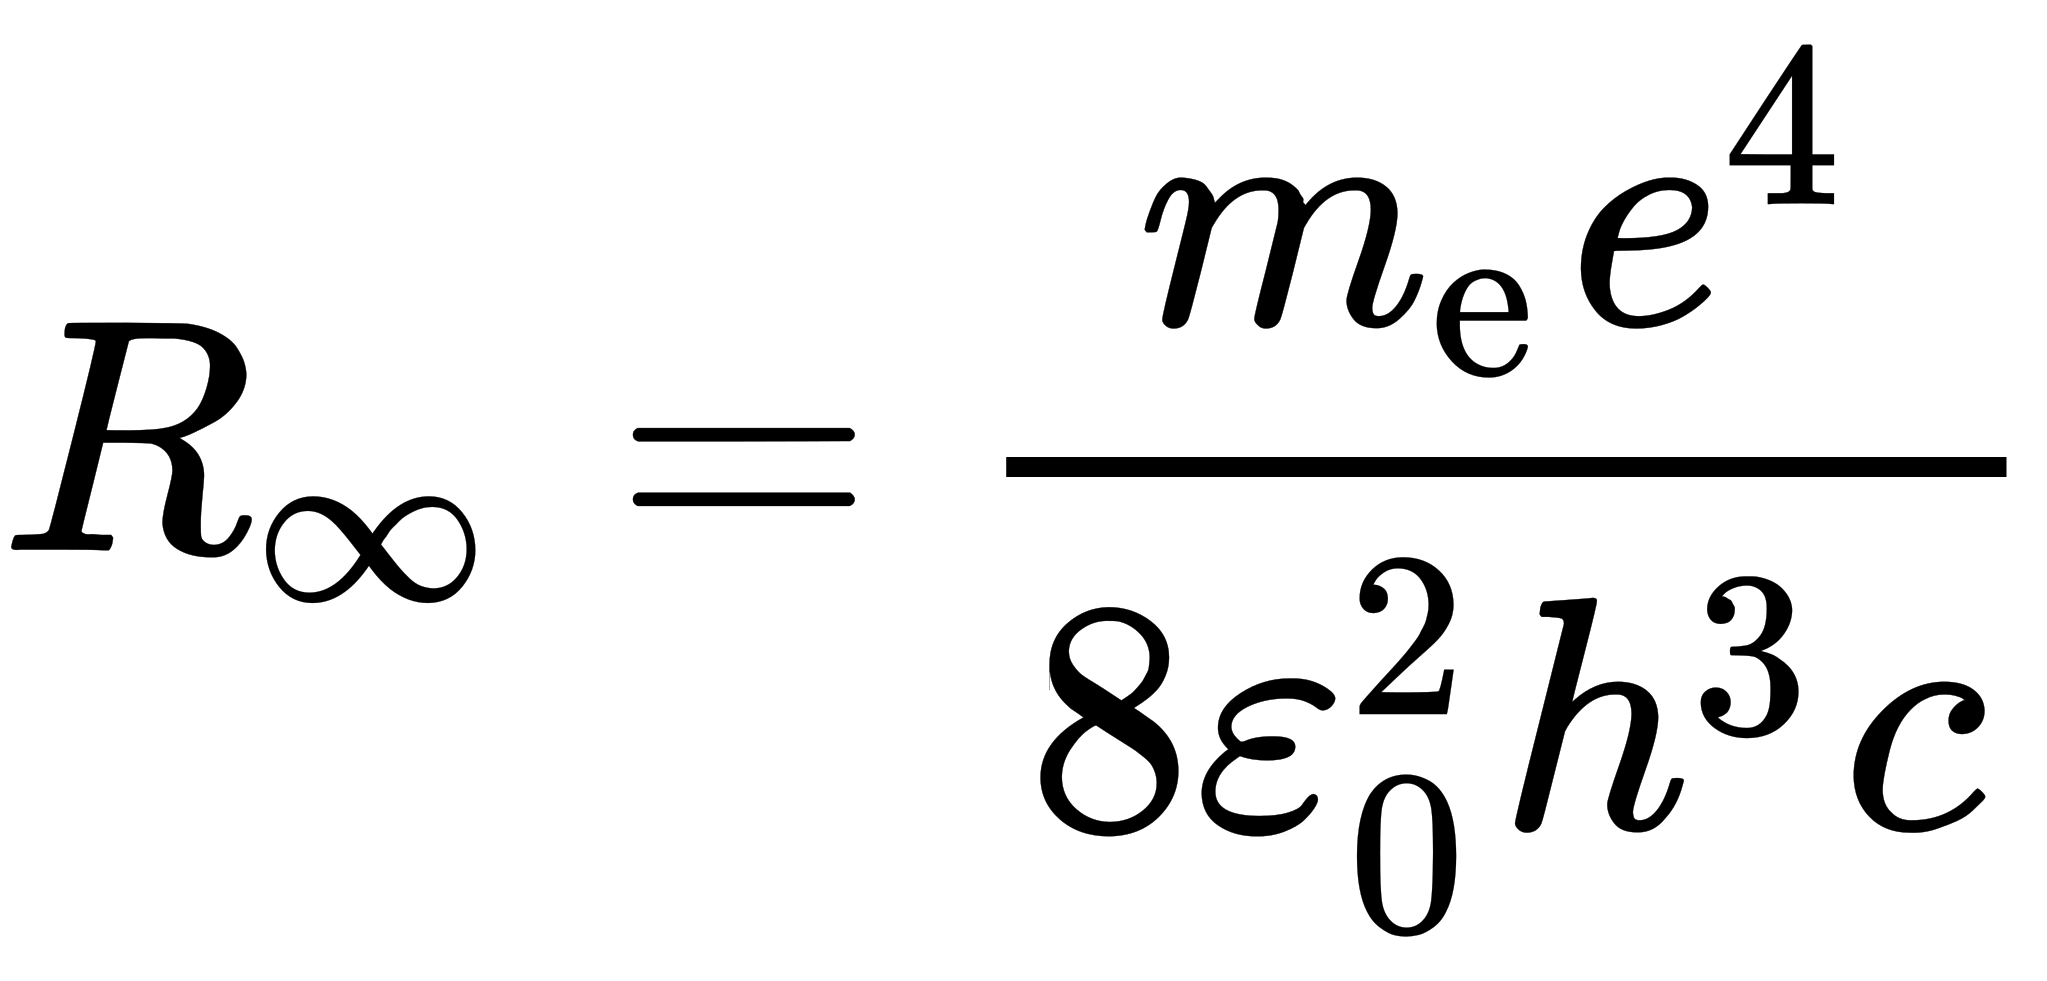
\includegraphics[scale=0.5]{1.png}
	\caption{ جدول داده های آزمایش تشعشع جسم سیاه در دماهای مختلف}
	\label{Fig1}
\end{figure}
  
   و بر اساس این جدول به رسم نمودار در اکسل پرداختم
   \footnote{توجه شود که در رسم این نمودار باز هم باید از رابطه شماره ۶ استفاده کرد چرا که فاصله ی دیافراگم و ترموپیل حدود ۵.۱۳ سانتی متر است و این باعث می شود که نتوانیم از رابطه ی ساده ی 
   $I = \sigma T^4$
   استفاده کنیم.
}
   ، فایل اکسلی که در آن این نمودار رسم شده است ضمیمه شده است. به این گراف برای شدت تابش بر حسب 
   $T^4$
   رسیدم: (شکل \ref{Fig2})
   
      \begin{figure}[h]
   	\centering
   	\includegraphics[scale=1]{2.jpg}
   	\caption{ نمودار شدت تابشی بر حسب توان چهارم دما}
   	\label{Fig2}
   \end{figure}
   
   
   \noindent \\
   اگر بخواهیم شیب خط این شکل را به عنوان ثابت استفان-بولتزمن تعبیر کنیم، یعنی اگر قرار دهیم که:
   \[
   \sigma = 8.37 \times 10^{-8} \frac{J}{m^2 .s .  K^4}
   \]
  که با دقت نسبتا خوبی ثابت استفان بولتزمن را به دست می دهد.
  \footnote{
توجه کنید که در فایل اکسل، دقت نمایش شیب و عرض از مبدا را تا ۲۰ رقم زیاد کرده ام ولی تمامی این رقم ها ارزش ندارند و سه رقم اول این شیب برای ما ارزشمند است.  
}
  
  \noindent
  توجه داشته باشید که مقدار عرض از مبدا این خط ناصفر است و به این دلیل است که دمای محیط هم ناصفر است و با کاستن این دما از مقدار 
  $T^4$
  می توان دید که عرض از مبدا هم صفر می شود، البته اینجا به این مقدار عرض از مبدا کاری نداریم.
  
  \noindent\\
  پس قادر بودیم که هم رابطه ی خطی بین شدت و توان چهارم دما را تحقیق کنیم و هم توانستیم ثابت استفان-بولتزمن را بدست آوریم؛ درصد خطای نسبی این مقدار برای 
  $\sigma$
   برابر 
   $-47\%$
   است.

\section{آزمایش دوم: تحقیق بستگی شدت به عکس مجذور فاصله }
در این آزمایش دمای محیط و دمای جسم سیاه را ثابت نگه می داریم و با حرکت دادن ترموپیل در فواصل مختلف نسبت به دیافراگم، داده های مختلفی را ثبت می کنیم و از روی آن می توانیم با داشتن پارامتر های دیگر [مانند دمای جسم سیاه و شعاع دیافراگم و جسم سیاه]، مقدار ثابت استفان بولتزمن را به دست آوریم.

\noindent\\
جدول داده های این آزمایش این چنین بود(شکل 
\ref{Fig3}
)
\begin{figure}[h]
	\centering
	\includegraphics[scale=0.6]{3.png}
	\caption{ داده های آزمایش تحقیق بستگی شدت به عکس مجذور فاصله}
	\label{Fig3}
\end{figure}

   و بر اساس این جدول به رسم نمودار در اکسل پرداختم، فایل اکسلی که در آن این نمودار رسم شده است ضمیمه شده است. به این گراف برای توان بر حسب 
   $r^{-2}$
   رسیدم (شکل 
   \ref{Fig4}
   )
   \begin{figure}[h]
   	\centering
   	\includegraphics[scale=1]{4.jpg}
   	\caption {توان رسیده به ترموپیل بر حسب عکس مجذور فاصله ترموپیل با دیافراگم }
   	\label{Fig4}
   \end{figure}

\noindent \\ 
حال قصد ما این است که ثابت استفان بولتزمن را از این گراف حاصل کنیم.

\noindent
 مطابق رابطه ی (۶) دستور کار که رابطه زیر است:
 \[
 R_T = \sigma(T^4 - T_0^4) = \frac{4\pi r^2}{2} \times \frac{1}{\pi (\frac{R_1}2)^2} \times
 \frac{W}{\pi (\frac{R_2}2)^2}
 \]
 
 می دانیم که نمودار بالا، نمودارِ 
 $W(\frac{1}{r^2})$
 است و شیب این خط مطابق رابطه ی (۶) برابر است با:
 \[
 \sigma(T^4 - T_0^4)\pi^2 (\frac{R_1}2)^2 (\frac{R_2}2)^2 \times \frac{2}{4\pi}
 \]
 
 حالا با داشتن شیب خط از روی شکل 
 \ref{Fig4}
 و داشتن دمای جسم سیاه (
 $388^{\circ}  C$
 ) 
 و دمای محیط 
 ( $18.5^{\circ}  C$)
و قطرهای دیافراگم و جسم سیاه (آن قسمتی که در معرض تابش است)
($R_1 = 0.025 m$ و 
$R_2 = 0.02 m$
)
می توانیم با جاگذاری در رابطه بالا، مقدار ثابت استفان بولتزمن را بخوانیم:
\[
\sigma((661)^4-(291.5)^4)(3.1415)^2(\frac{0.02}{2})^2(\frac{0.025}{2})^2\times \frac{1}{2\pi} = 0.000364
\]
\[
\sigma = 8.07 \times 10^{ -8}\frac{J}{m^2 .s .  K^4}
\]
که نسبتا با ثابت استفان بولتزمان همخوانی دارد.

\noindent
و مقدار درصد خطای نسبی این آزمایش برابر با 
$-42\% $
است و این خطا اگر چه باز هم زیاد است، ولی باز ما را به مقدار حقیقی این ثابت نزدیک تر کرده است.



\section{سوالات}
\subsection{سوال یک}
چرا از جریان آب برای خنک کردن دهانه کوره استفاده شد؟

\noindent\\
ممکن است که تابش های دهانه ی کوره از دیافراگم عبور کند و توسط ترموپیل جذب شود و در نتیجه آزمایش خطا ایجاد کند پس بهتر است که در حد امکان اطراف دهانه کوره را خنک کنیم و در ضمن بدنه کوره هم برای ایمنی بیشتر آزمایشگران در مقابل خطاهای سهوی توسط آب خنک می شود. به این علت از آب استفاده می شود که در دسترس ترین مایع است و بالاترین ظرفیت گرمایی را داراست.

\subsection{سوال دو}
منحنی $W$‌را بر حسب  
$\frac{1}{r^2}$
رسم کنید و از طریق آن ثابت استفان بولتزمن را بدست آورید.

\noindent\\
 این همان کاری است که در بخش دوم این گزارش انجام شده است.
 

\subsection{سوال سه}
توضیح دهید چرا منحنی سوال ۲ از مبدا نمی گذرد؟

\noindent\\

مطابق رابطه ی (۶)، این ها بایستی از مبدا بگذرند ولی در انجام این آزمایش خطاهایی هست که اجتناب از آن ها به طور کامل امکان پذیر نیست؛ از جمله:
\begin{itemize}
	\item چون آن قسمتی از جسم سیاه که تابش می کند در تماس با خنک کننده است، پس دمای قرصی که تابش می کند، تماما یکسان نیست و مقدار آن به صورت شعاعی تغییر می کند، پس این باعث تولید خطا در نتیجه می شود.
	\item این استوانه ای که در کوره قرار دارد، جسم سیاه کامل نیست و آن چه که توسط ما اندازه گیری می شود، دقیقا مقدار ثابت استفان بولتزمن نیست بلکه ضریب جذب در ثابت است یعنی 
	$\epsilon\sigma$
	\item هر گونه اغتشاشاتی در جریان هوای اطراف، مانند حرکت یک انسان، باعث می شود که طیف تابشی توسط ترموپیل با خطایی محاسبه بشود.
	\item دستگاه های استفاده شده در سیستم خود دارای دقت اندازه گیری محدود هستند
\end{itemize}
 
 همین موارد باعث ایجاد یک خطا در شیب خط یا عرض از مبدا شده اند.

\subsection{سوال چهار}
$\lambda_{max}$
برای بدن انسان چقدر است؟ اگر 
$\lambda_{max}$
برای خورشید 5100 آنگستروم و برای ستاره ی شمالی 3500 آنگستروم باشد، دمای هر کدام چقدر است؟
\noindent\\
از قانون جابه جایی وین استفاده می کنیم:
\[
\lambda_{max}T = 2.9\times 10^{-3} m.K
\]
با جای گذاری دمای بدن انسان که حدود ۳۱۰ درجه کلوین است؛ طول موج ماکسیمم بدن انسان
$9.35\times 10^{-6} m$
بدست می آید که در ناحیه فروسرخ است.

مشابها با جایگذاری هایی در رابطه بالا، دمای خورشید و دمای ستاره شمالی به ترتیب ۵۶۸۶ درجه کلوین و ۸۲۸۵ درجه کلوین هستند
\subsection{سوال پنج}
انحراف از معیار ثابت استفان بولتزمان را با استفاده از نتایج آزمایش اول به دست آورید و بازه تغییرات سیگما را گزارش دهید؛ یعنی 
$\sigma \pm A.D$

\noindent\\
در فایل اکسل یک ستون مربوط به مقادیر ثابت استفان بولتزمن برای هر داده است و در خانه ی زیرین آن مقدار انحراف معیار را بدست آورده ایم:
\[
\sigma =  8.37 \times 10^{-8} \pm 2.01\times 10^{-9} \frac{J}{m^2 .s .  K^4} 
\]
\subsection{سوال شش}
چگونه می توان با استفاده از نتایج آزمایش، تصویربرداری حرارتی کرد؟

\noindent\\
از همین آزمایش نتیجه های خوبی در مورد این که شدت تابش با فاصله از منبع تابش دارد، و شیوه ی ارتباط شدت تابش با دما گرفتیم، پس اگر یک ترموپیل داشته باشیم، یعنی وسیله ای داشته باشیم که شدت نور را بتواند تشخیص دهد، و همچنین بتوانیم فاصله را از چشمه نور تعیین کنیم، و با داشتن دو پارامتر مربوط به قطر دیافراگم و ترموپیل، می توانیم دمای جسم را بخوانیم و با مجموعه ی نکات مطرح شده در این آزمایش به تصویربرداری حرارتی دست بیابیم.
 

\subsection{سوال هفت}
رابطه (۶) را ثابت کنید.

\noindent\\
در این ست آپ، جسم سیاه منبع تابش است و در نزدیکی دیافراگم، رابطه زیر را بین شدت و توان داریم:
\[
\sigma(T^4-T_0^4) = \frac{P_s}{\pi(\frac{R_d}2)^2}
\]
که در آن 
$R_d$
همان قطر دیافراگم است و
$P_s$
همان توان منبع است.


حالا برای یافتن توان در  نقطه ای که ترموپیل قرار دارد از رابطه ی 
$I = \frac{P_{tot}}{4\pi r^2}$
استفاده کرد:

\[
P_{t} = \frac{P_s}{\frac42\pi r^2} \times \pi (\frac{R_t}{2})^2
\]
این رابطه به سادگی می گوید که توان در محل ترموپیل، توان کل تقسیم بر سطح کره ای به شعاع 
$r$
 است، اما ضریب یک دوم به این خاطر است که این تابش روی یک نیم کره پخش می شود، و با ضرب کردن در سطح ترموپیل ، توانی که ترموپیل دریافت می کند را پیدا می کنیم، حال اگر از بالا برای 
 $P_s$
 را جایگذاری کنیم.
 \[
 P_t = \frac{\sigma(T^4 - T_0^4)}{2\pi r^2} \times \pi (\frac{R_t}{2})^2 \times \pi (\frac{R_d}{2})^2
 \]
و این همان رابه (۶) است. پس اثبات کامل است.






\end{document}